\documentclass[subsection=false]{beamer}
\setbeamertemplate{footline}[frame number] % numerar slides
\setbeamertemplate{navigation symbols}{} % retirar barra de navega��o

\mode<presentation>
\usetheme{Singapore}

\ifdefined\hyperref  

\usepackage[brazil]{babel}
\usepackage[latin1]{inputenc}
\usepackage{graphicx}
\usepackage{subcaption}  
\usepackage{pgfpages}
\usepackage{ifpdf}   
\usepackage{multimedia}  
\usepackage{color}   
\usepackage{url} 
\usepackage{hyperref}
\usepackage{lastpage}

\pgfdeclareimage[width=0.85cm, height=1.10cm]{ufpa}{Figures/logo_ufpa}
\logo{\pgfuseimage{ufpa}}

\hypersetup{
	pdftitle={ASR e TTS Embarcado para Controle de TV}
	pdfauthor={Cassio Trindade Batista}
}
\fi

\title[ASR + TTS: Controle de Equipamentos Eletr�nicos\hspace{2.10cm}\thepage/\pageref{LastPage}]
{Uso de Reconhecedor e Sintetizador de Voz para Controle de Equipamentos Eletr�nicos}

\author[Cassio, Pedro, Gabriel e Thiago]{\small
Cassio Trindade Batista\\
Gabriel Peixoto de Carvalho\\
Pedro Henrique C. F. Soares\\
Thiago Barros Coelho}

\institute{\scriptsize
Universidade Federal do Par�\\
Instituto de Tecnologia\\
Faculdade de Engenharia da Computa��o e Telecomunica��es\\
Disciplina: Projetos de Hardware e Interfaceamento\\
Professores: Jeferson Leite e Adalbery Castro\\
\begin{figure}
	
\includegraphics[width=.13\textwidth]{Figures/logo_ufpa}
\end{figure}
\vspace{-.5cm}
}
\date{\small{30 de maio de 2015}}

\begin{document}
\begin{frame}[plain]
	\titlepage
\end{frame}

\section{Introdu��o}
\begin{frame}{Introdu��o}
\end{frame}

\begin{frame}{ASR vs TTS}
\begin{figure}
	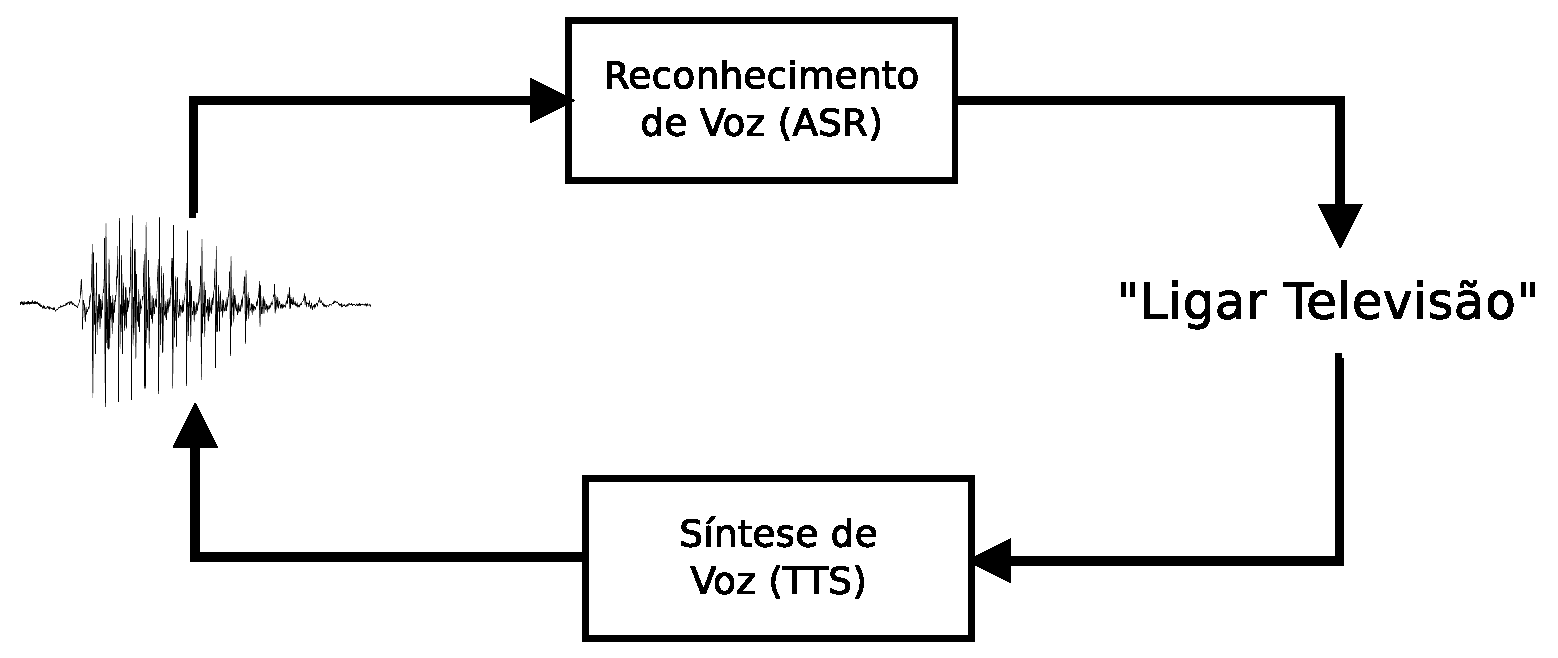
\includegraphics[width=\textwidth]{Figures/asr_tts}
\end{figure}
\end{frame}

\begin{frame}{ASR vs TTS}
\begin{figure}
	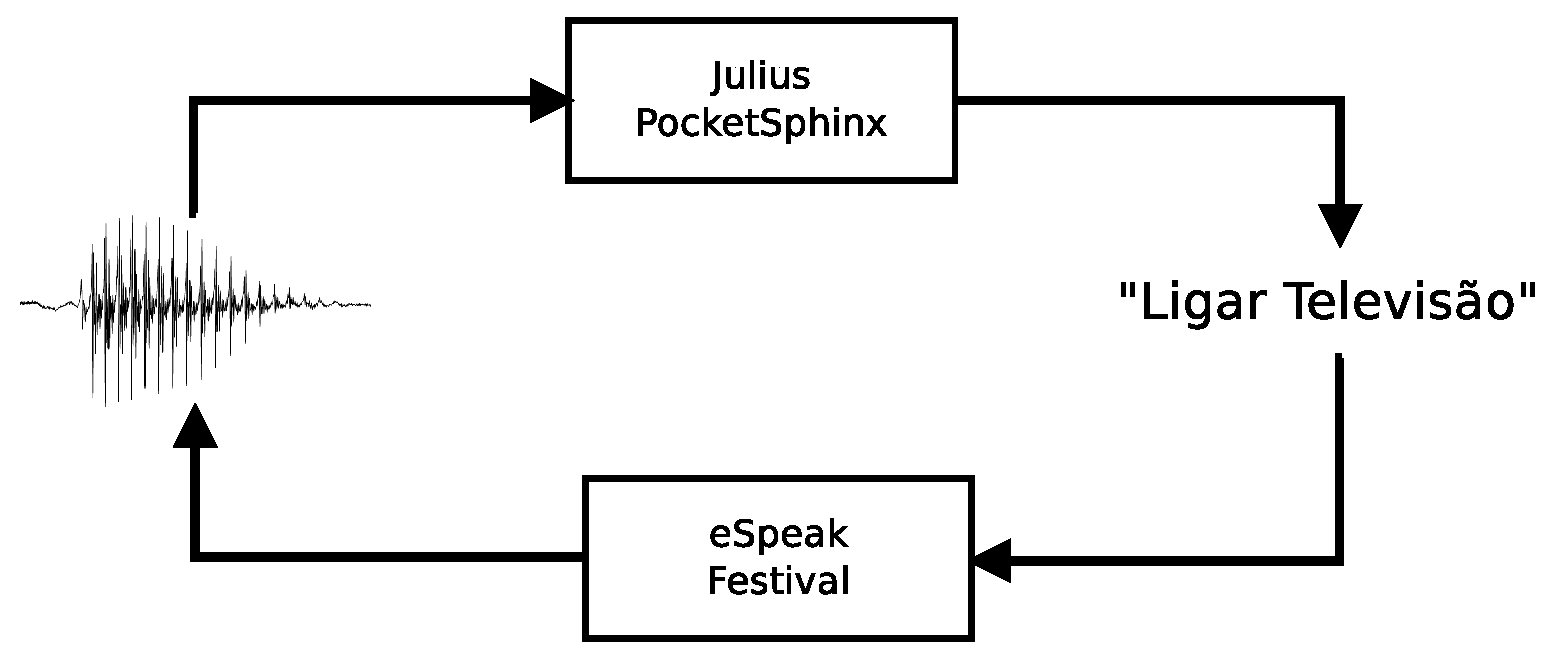
\includegraphics[width=\textwidth]{Figures/asr_tts_soft}
\end{figure}
\end{frame}

\begin{frame}{Reconhecimento Autom�tico de Voz}
\begin{figure}
	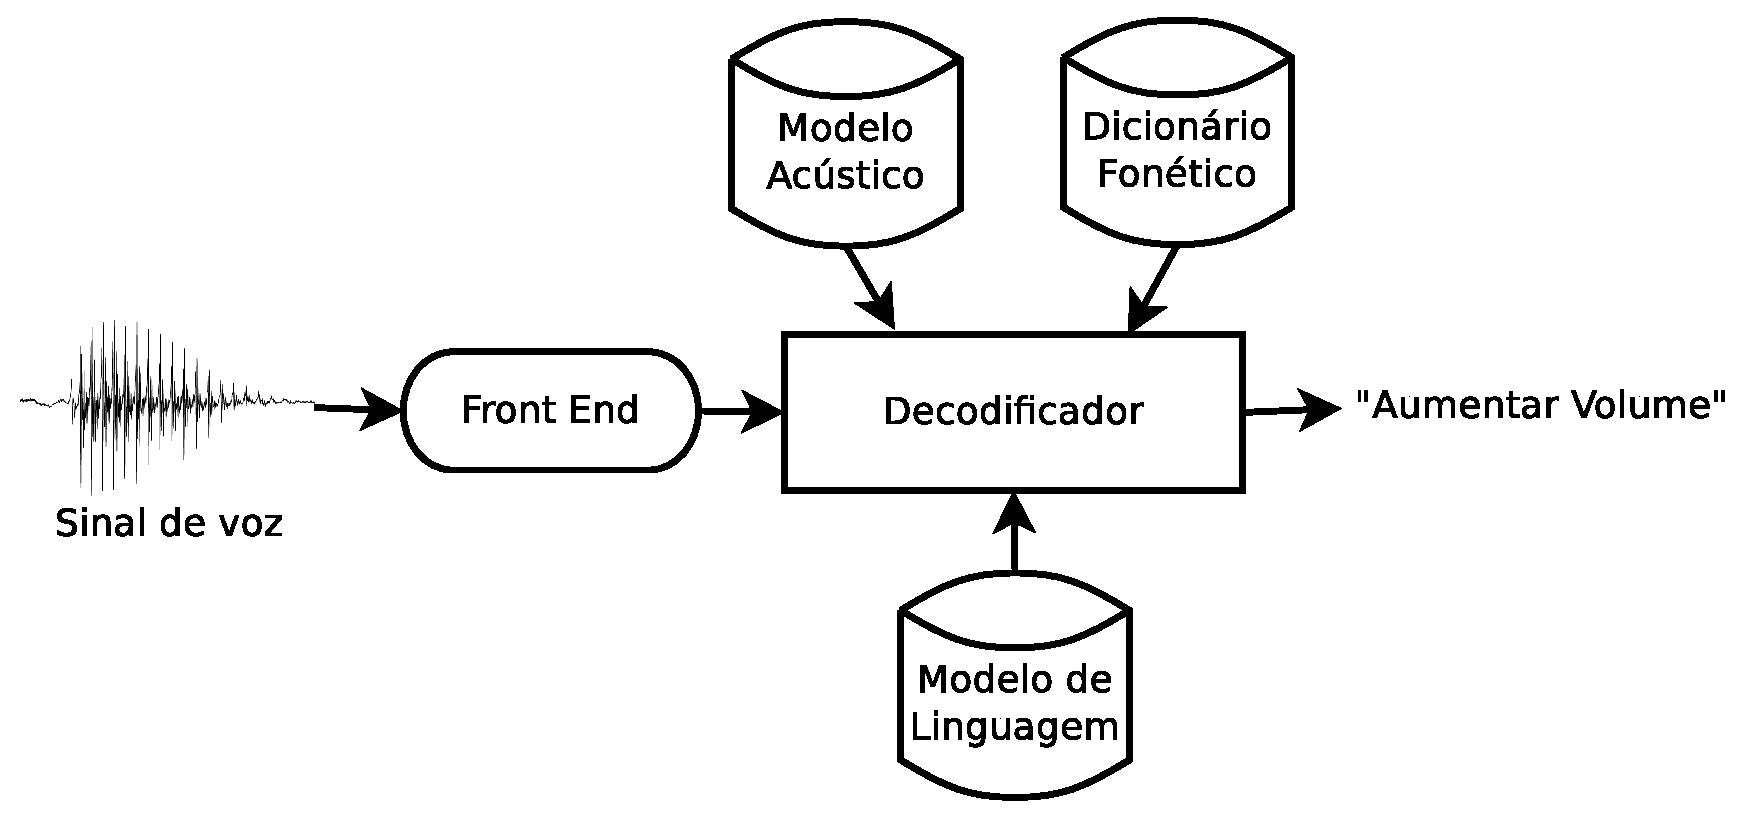
\includegraphics[width=\textwidth]{Figures/asr_sch}
\end{figure}
\end{frame}

\begin{frame}{Beagle Beagle Beagle}
\begin{figure}
	\includegraphics[width=\textwidth]{Figures/schematic}
\end{figure}
\end{frame}

\begin{frame}{Philips RC-5 Protocol}
\begin{figure}
	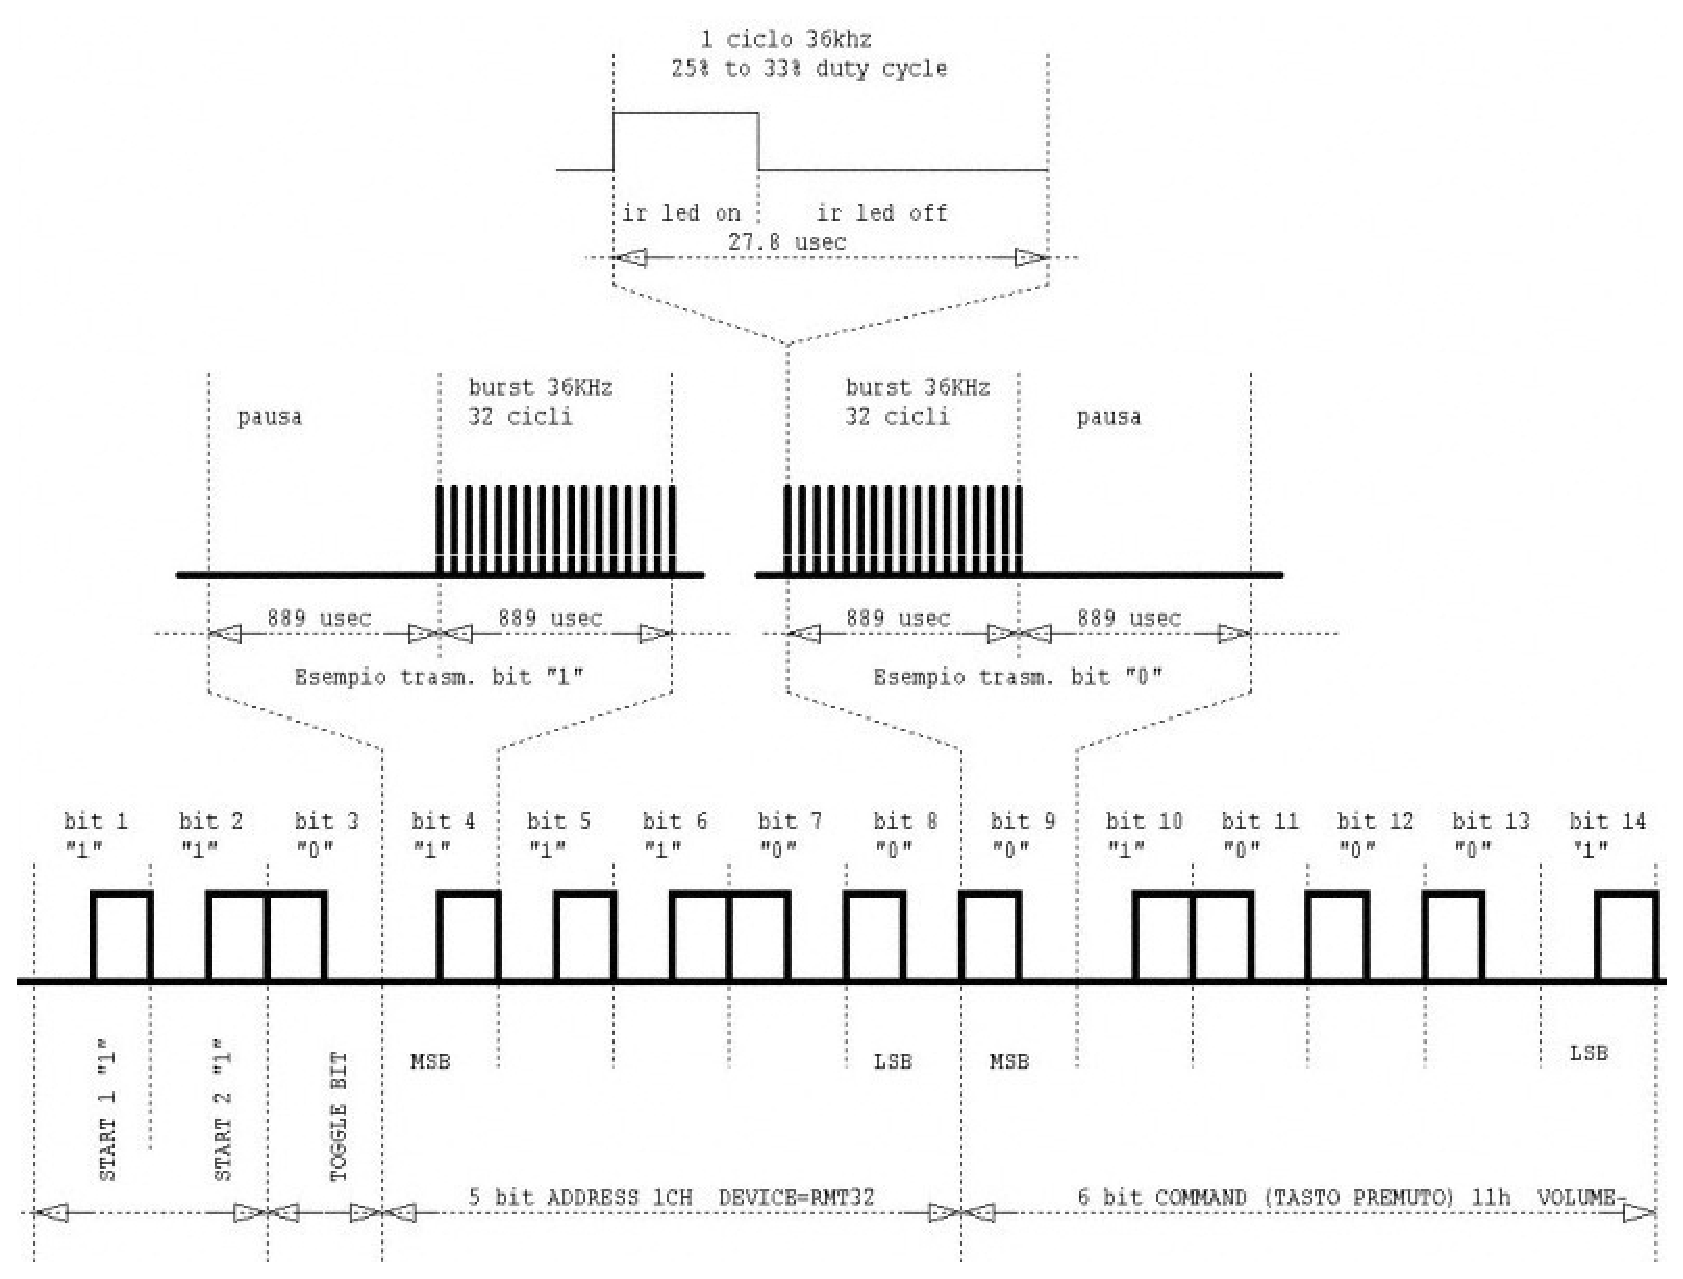
\includegraphics[width=.9\textwidth]{Figures/sch_rc5}
\end{figure}
\end{frame}

\begin{frame}{Vlw Flw!}
\end{frame}
\end{document}
%%% EOF %%%
